\documentclass{ctexart}
\usepackage{amsmath}
\usepackage{graphicx}
\usepackage{float}
\usepackage{geometry}
\usepackage{hyperref}
\usepackage{tabularx}
\title{弗兰克-赫兹实验实验报告}
\author{陈启钰\,\,\, 2300011447}
\date{\today}
\begin{document}
	\maketitle
	\section{数据处理}
	\subsection{汞管}
	实验测量汞管时各参量设置为
	\begin{align}
		U_1=1.51\mathrm{V},U_3=1.88\mathrm{V},T=178^\circ\mathrm{C}
	\end{align}
	各参量的物理意义如图\ref{meaning1}所示
	\begin{figure}[H]
		\centering
		\includegraphics[width=0.5\linewidth]{meaning1.jpg}
		\caption{参数示意图}
		\label{meaning1}
	\end{figure}
	通过测量输出电压$U_{\mathrm{out}}$和$U_2$的关系,得到图\ref{u3199}
	\begin{figure}[H]
		\centering
		\includegraphics[width=0.6\linewidth]{u3199.png}
		\caption{$U_{\mathrm{out}}-U_2$关系图}
		\label{u3199}
	\end{figure}
	\subsection{氩管}
	实验测量氩管的各参量设置为
	\begin{align}
		V_{\mathrm{HH}=3.0\mathrm{V}},V_{\mathrm{G_2A}}=6.5\mathrm{V},V_{\mathrm{G_1K}}=2.0\mathrm{V}
	\end{align}
	各参量的物理意义如图\ref{meaning2}所示
	\begin{figure}[H]
		\centering
		\includegraphics[width=0.5\linewidth]{meaning2.jpg}
		\caption{参数示意图}
		\label{meaning2}
	\end{figure}
	通过测量$I_{\mathrm{out}}$和$V_{\mathrm{G_2K}}$关系,可得图\ref{ar}
	\begin{figure}[H]
		\centering
		\includegraphics[width=0.6\linewidth]{ar.png}
		\caption{$I_{\mathrm{out}}-V_{\mathrm{G_2K}}$关系图}
		\label{ar}
	\end{figure}
	\section{第一激发电位的测量}
	根据所得的实验数据,将六个峰值列表如下
	\begin{table}[H]
		\begin{center}
			\caption{汞管和氩管的峰值扫描电压}
			\begin{tabular}{c|cccccc}
				$n$&1&2&3&4&5&6\\
				\hline
				$U_{\mathrm{Hg}}/\mathrm{V}$&4.8&9.5&14.4&19.1&24.0&28.9 \\
				\hline
				$U_{\mathrm{Ar}}/\mathrm{V}$&15.9&27.5&39.4&51.9&65.2&78.2\\
				\hline
			\end{tabular}
		\end{center}
	\end{table}
	用最小二乘法进行线性拟合,得到
	\begin{align}
		U_{\mathrm{Hg}}=nU_{\mathrm{Hg1}}+U_{\mathrm{Hg0}}\\
		U_{\mathrm{Ar}}=nU_{\mathrm{Ar1}}+U_{\mathrm{Ar0}}
	\end{align}
	其中
	\begin{align}
		U_{\mathrm{Hg1}}=4.82\mathrm{V},U_{\mathrm{Hg0}}=-0.0867\mathrm{V},r_{\mathrm{Hg}}=0.99997\\
		U_{\mathrm{Ar1}}=12.49\mathrm{V},U_{\mathrm{Ar0}}=2.64\mathrm{V},r_{\mathrm{Ar}}=0.9996
	\end{align}
	根据不确定度公式
	\begin{align}
		\frac{\sigma_k}{k}=\sqrt{\frac{\frac{1}{r^2}-1}{n-2}}
	\end{align}
	计算得到
	\begin{align}
		U_{\mathrm{Hg1}}=(4.82\pm0.02)\mathrm{V}\\
		U_{\mathrm{Ar1}}=(12.49\pm0.18)\mathrm{V}
	\end{align}
	\section{选做部分}
	此处采用汞管进行实验。
	
	改变反向电压$U_3$,测量后两个峰谷,可得图\ref{comparison}
	\begin{figure}[H]
		\centering
		\includegraphics[width=0.6\linewidth]{comparison.png}
		\caption{改变$U_3$大小时汞管后两个峰的改变}
		\label{comparison}
	\end{figure}
	可见,当增加$U_3$的值的时候,输出电压会变小,峰值降低且峰会右移。
	\section{思考题}
	改变减速电压的时候,相当于控制了电子到达阴极板的数量,当减速电压越大,电子到达阴极板所需的动能越高,也就是说能够到达阴极板的电子数量会减少,导致输出电流(电压)降低。此外,由于反向电压增大,电子需要更大的动能到达阴极,所以峰会右移图\ref{comparison}很好地验证了这一解释。
	\section{讨论}
	\subsection{曲线的特征}
	根据图\ref{u3199}和图\ref{ar}可以看出,输出电压(电流)有周期性,相邻两个峰对应的电压差就是各自原子对应的第一激发电位。随着可变电压(横轴)的增大,在电子尚未达到可以与原子碰撞并产生激发态前,输出电压(电流)会增大,直到电子动能达到某个特定值可以激发相应的原子,此时碰撞过后的电子动能减小,不能到达阴极,宏观上观察到的就是输出电压(电流)的减小,然后以此为周期发展。
	
	我们还可注意到峰值越来越大,这是因为总会有一部分电子不会与原子发生碰撞,以及,在能量足够高的情况下,碰撞过一次的电子仍有足够的动能到达阴极。所以峰值(当然还有谷值)都会增加。
	\subsection{测量第一激发电位的误差来源}
	随着实验的进行,电路各元件的温度会升高,而温度变化可能会对仪器造成影响,从而导致误差。
	
	此外,实验中输出电压(电流)的不稳定也可能造成误差。在进行实验的过程中也并没有等到稳态才进行读数,而是在调节电压2-3秒后就立即读数。
	\newpage
	\section{原始数据}
	\begin{figure}[H]
		\centering
		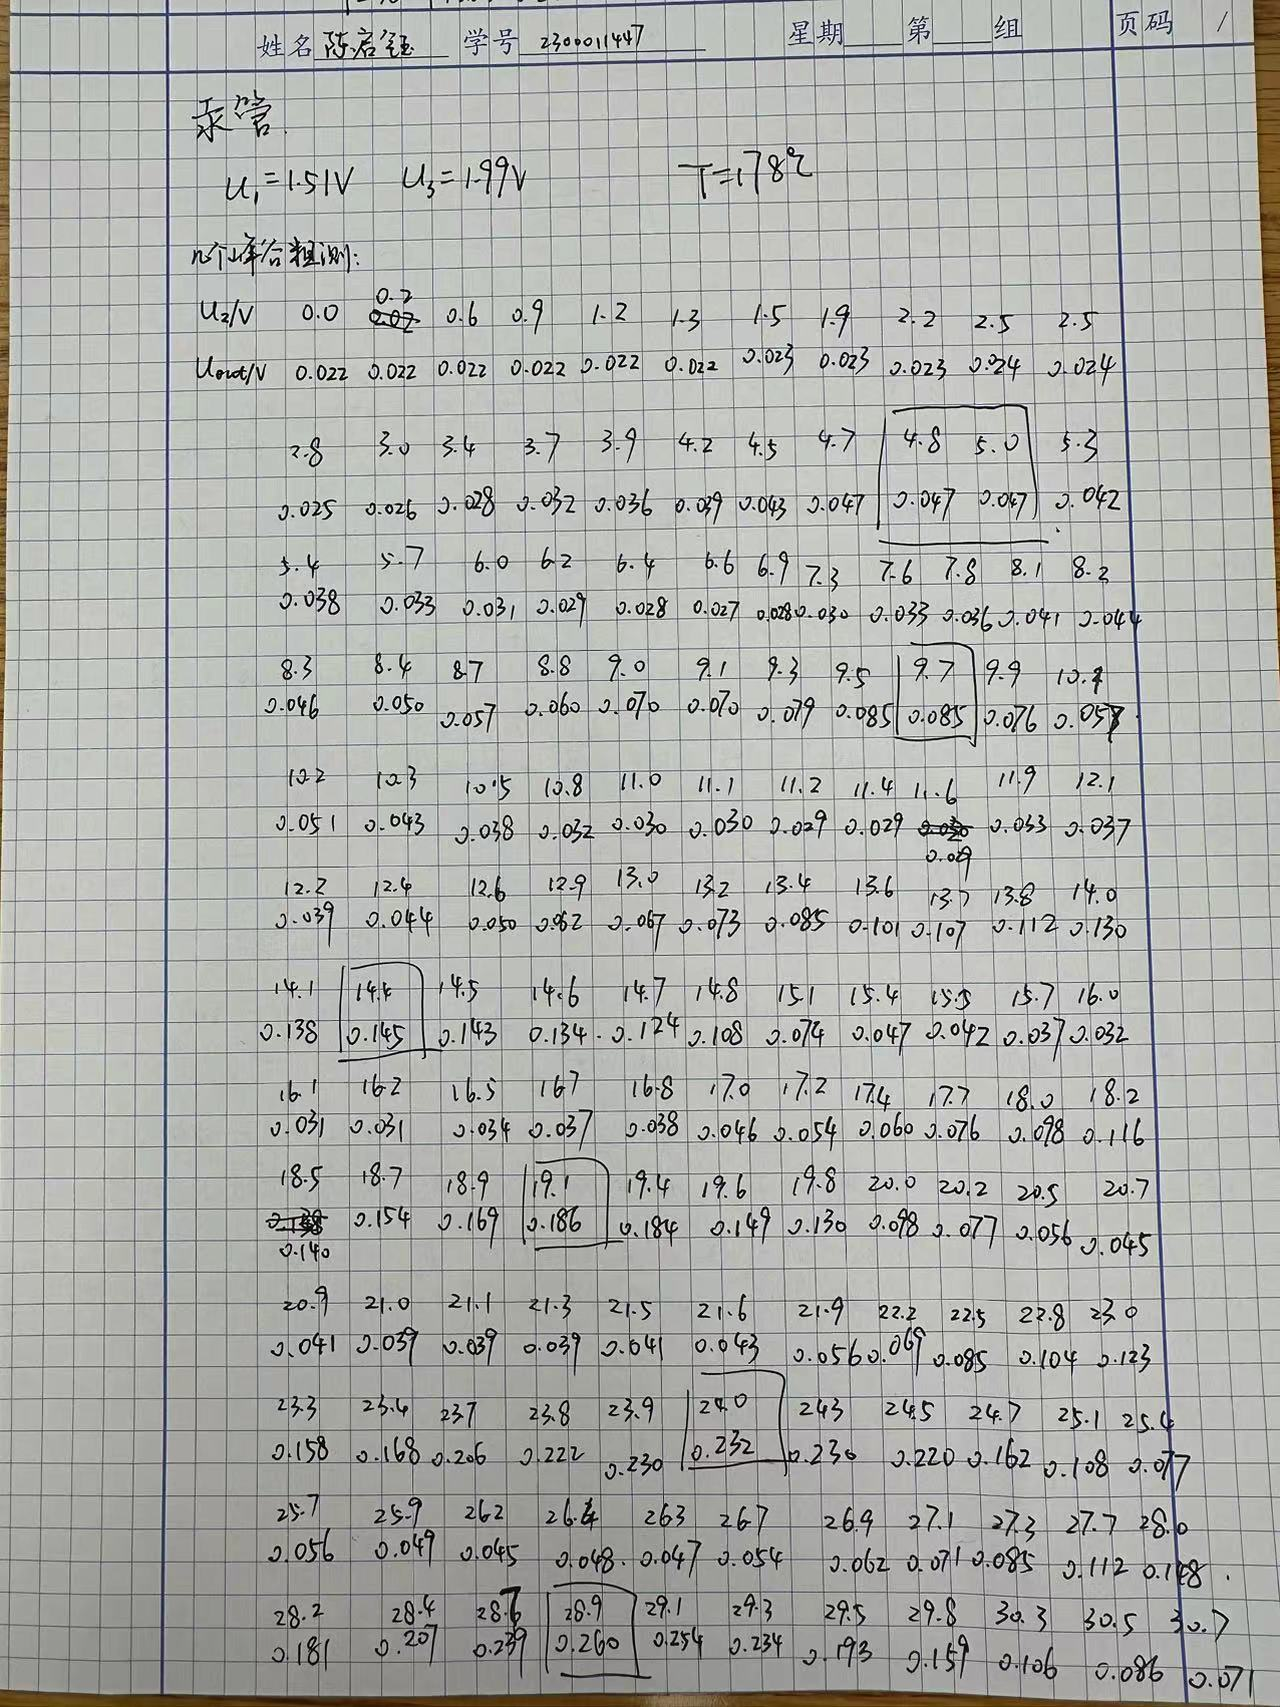
\includegraphics[width=0.6\linewidth,angle=270]{data1.jpg}
	\end{figure}
	\begin{figure}[H]
		\centering
		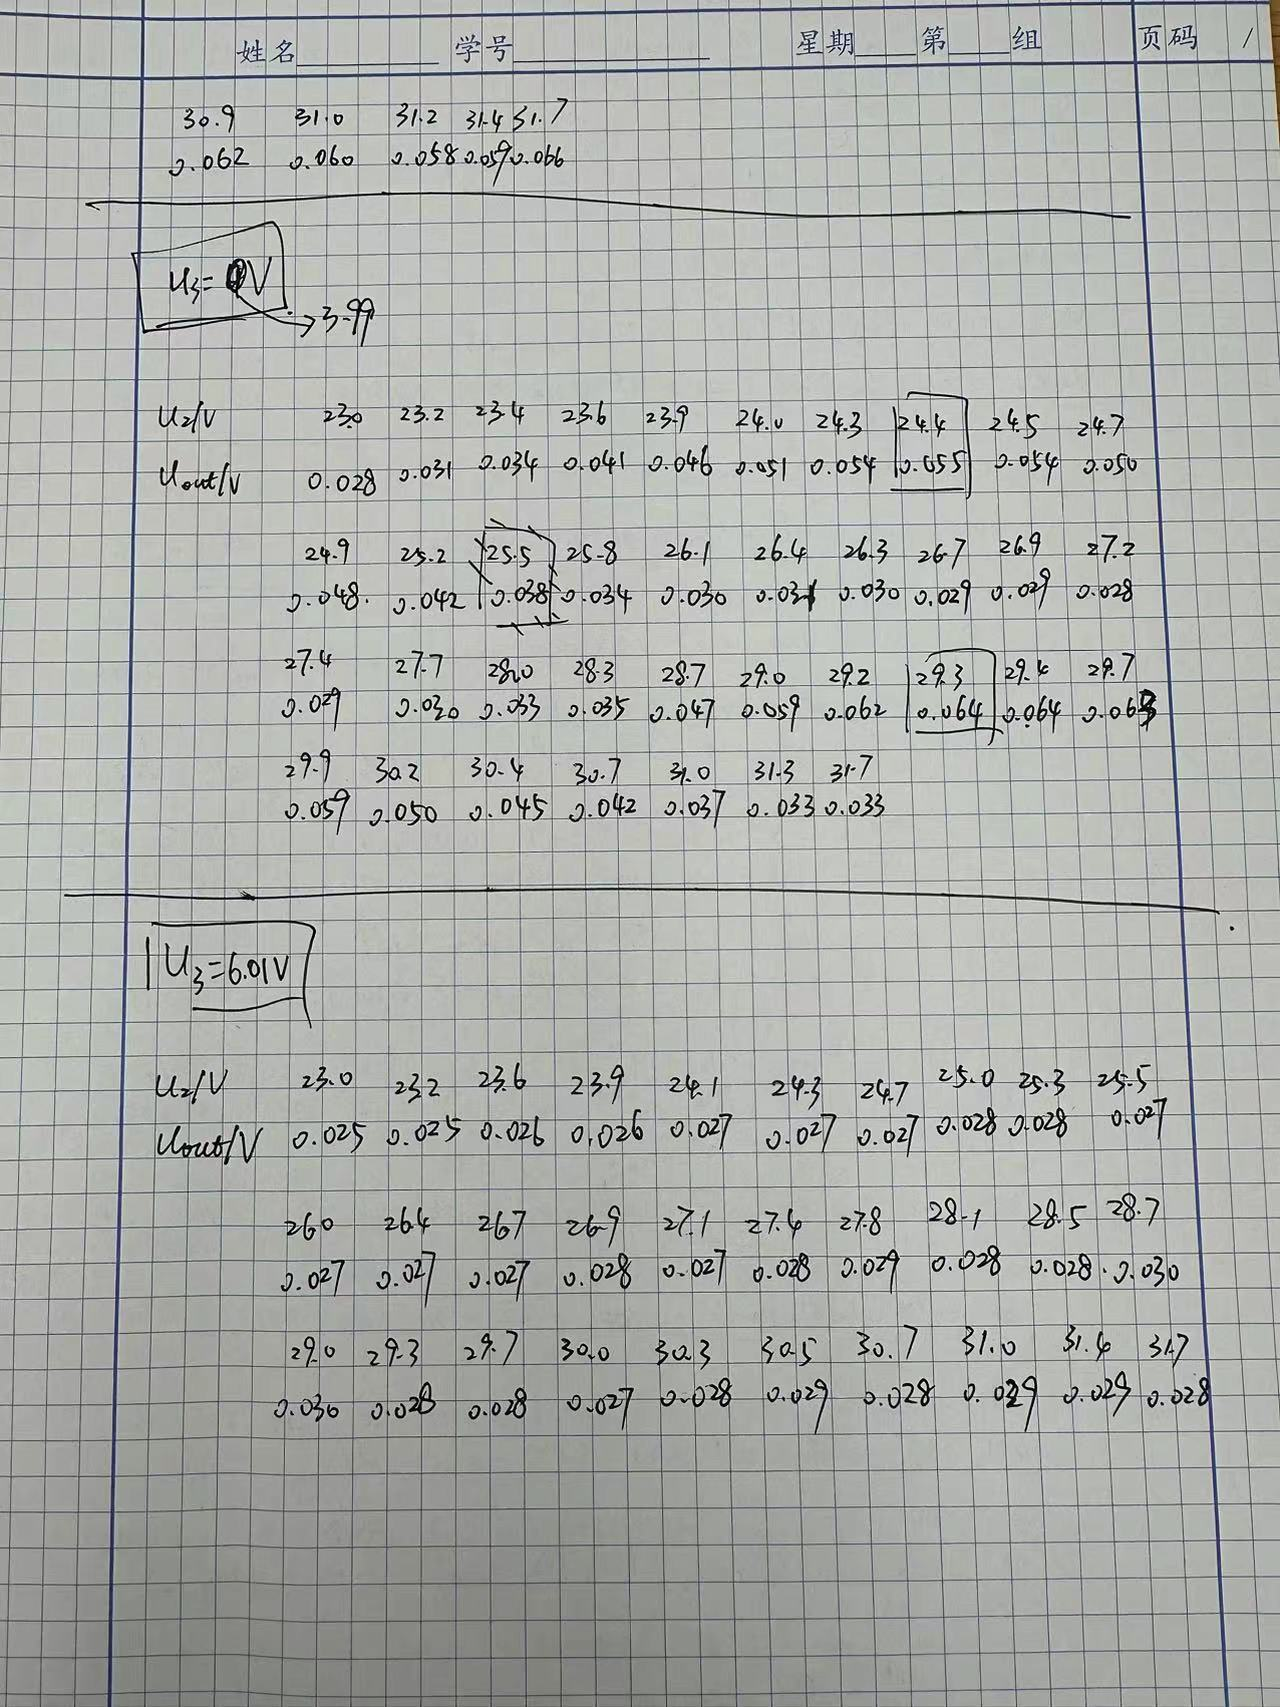
\includegraphics[width=0.6\linewidth,angle=270]{data2.jpg}
	\end{figure}
	\begin{figure}[H]
		\centering
		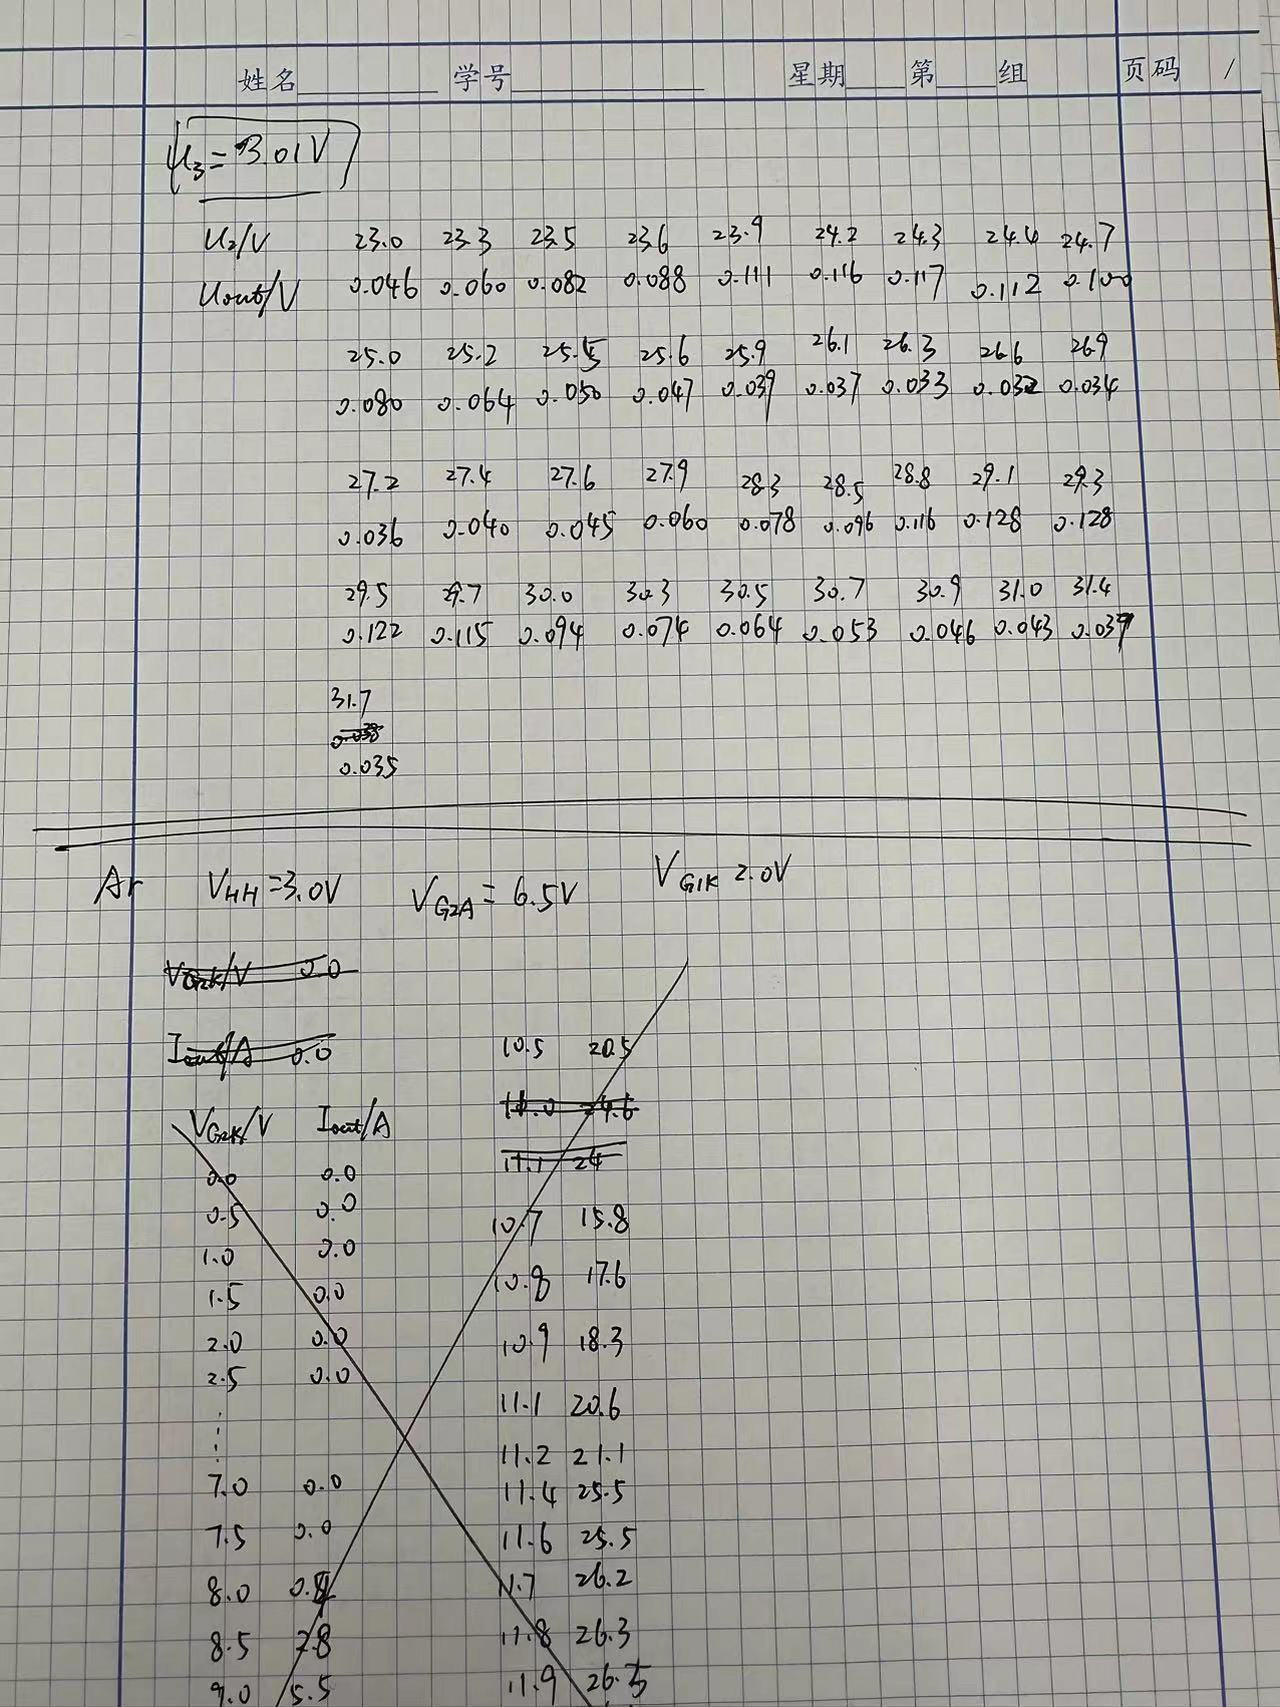
\includegraphics[width=0.6\linewidth,angle=270]{data3.jpg}
	\end{figure}
	\begin{figure}[H]
		\centering
		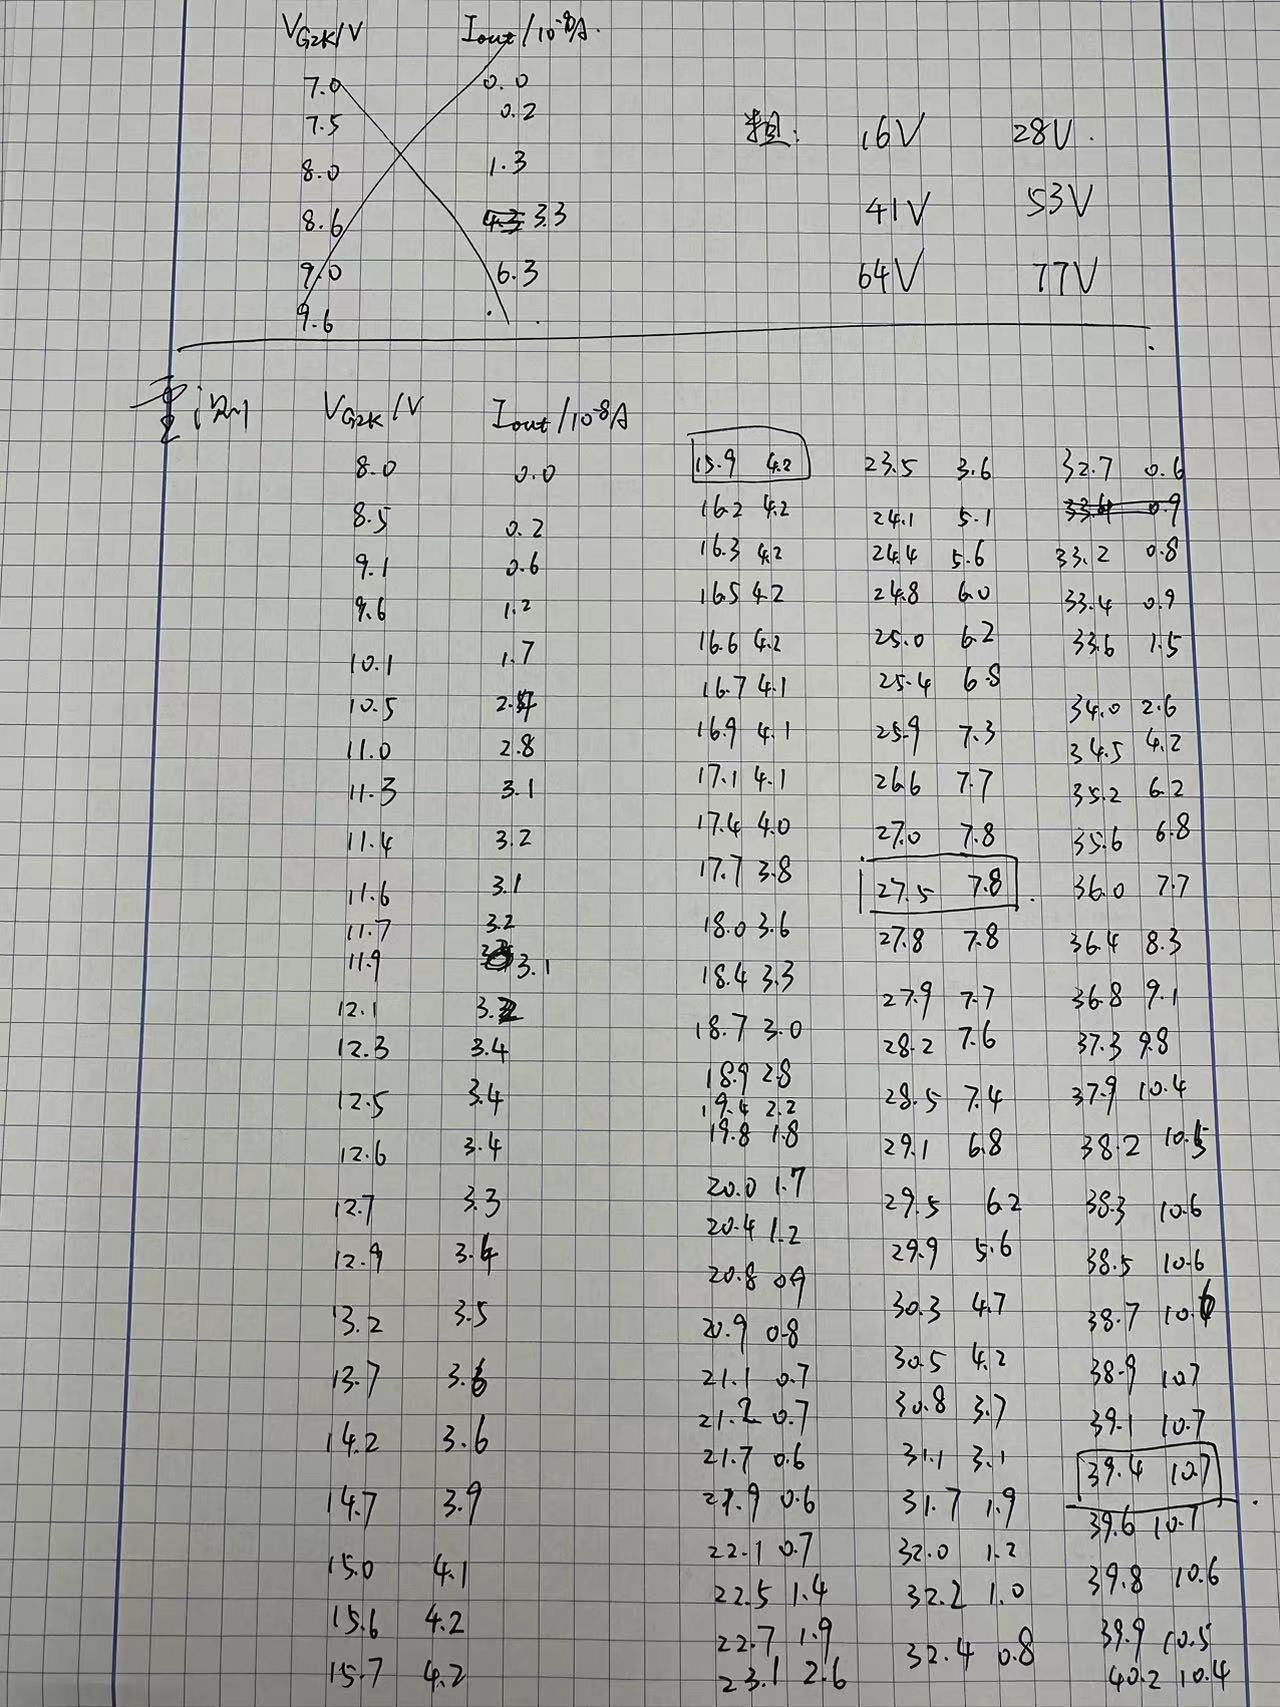
\includegraphics[width=0.6\linewidth,angle=270]{data4.jpg}
	\end{figure}
	\begin{figure}[H]
		\centering
		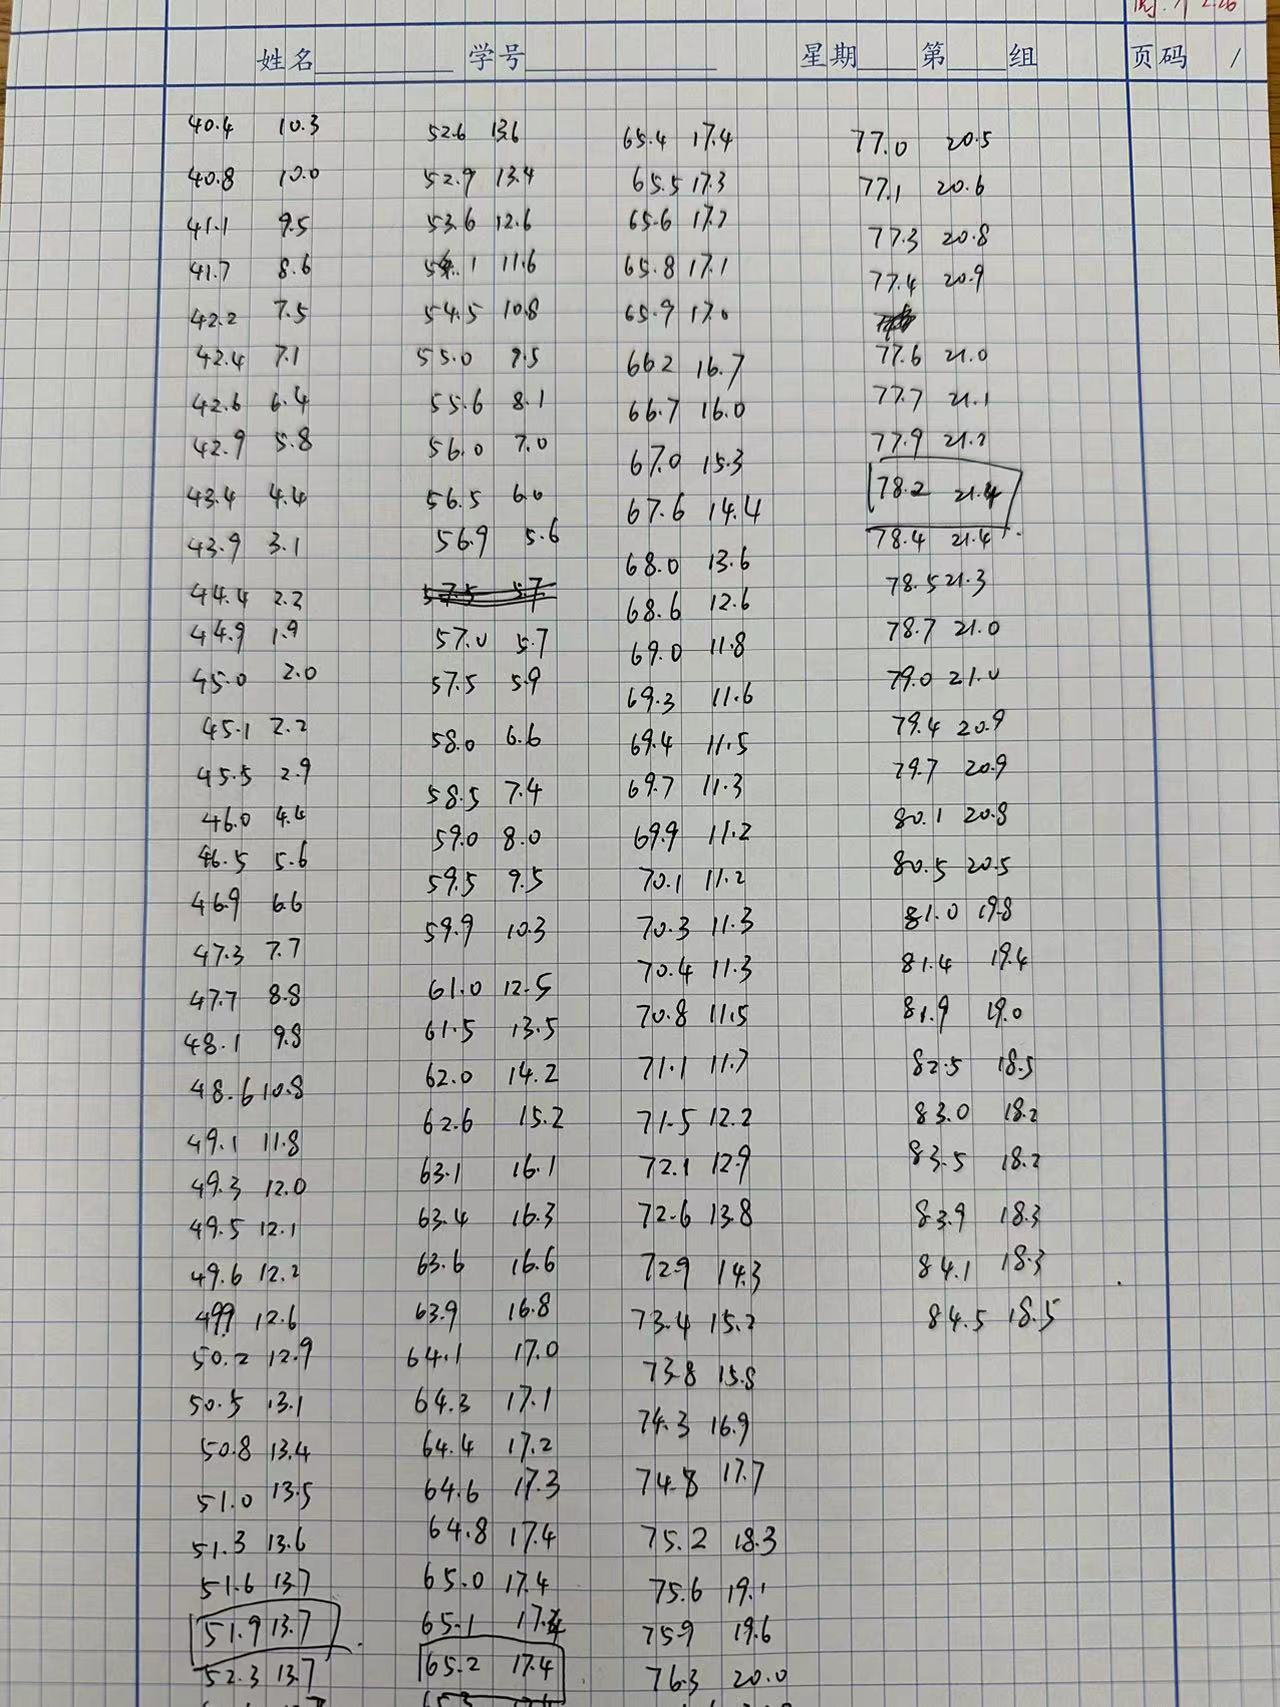
\includegraphics[width=0.6\linewidth,angle=270]{data5.jpg}
	\end{figure}
\end{document}